% !TEX encoding = UTF-8 Unicode
%%%%%%%%%%%%%%%%%%%%%%%%%%%%%%%%%%%%%%%%%
% Beamer Presentation
% LaTeX Template
% Version 1.0 (10/11/12)
%
% This template has been downloaded from:
% http://www.LaTeXTemplates.com
%
% License:
% CC BY-NC-SA 3.0 (http://creativecommons.org/licenses/by-nc-sa/3.0/)
%
%%%%%%%%%%%%%%%%%%%%%%%%%%%%%%%%%%%%%%%%%

%----------------------------------------------------------------------------------------
%	PACKAGES AND THEMES
%----------------------------------------------------------------------------------------

\documentclass{beamer}

\mode<presentation> {

% The Beamer class comes with a number of default slide themes
% which change the colors and layouts of slides. Below this is a list
% of all the themes, uncomment each in turn to see what they look like.

%\usetheme{default}
%\usetheme{AnnArbor}
%\usetheme{Antibes}
%\usetheme{Bergen}
%\usetheme{Berkeley}
%\usetheme{Berlin}
%\usetheme{Boadilla}
%\usetheme{CambridgeUS}
%\usetheme{Copenhagen}
%\usetheme{Darmstadt}
%\usetheme{Dresden}
%\usetheme{Frankfurt}
%\usetheme{Goettingen}
%\usetheme{Hannover}
%\usetheme{Ilmenau}
%\usetheme{JuanLesPins}
%\usetheme{Luebeck}
%\usetheme{Madrid}
%\usetheme{Malmoe}
%\usetheme{Marburg}
%\usetheme{Montpellier}
%\usetheme{PaloAlto}
%\usetheme{Pittsburgh}
%\usetheme{Rochester}
%\usetheme{Singapore}
%\usetheme{Szeged}
\usetheme{Warsaw}

% As well as themes, the Beamer class has a number of color themes
% for any slide theme. Uncomment each of these in turn to see how it
% changes the colors of your current slide theme.

%\usecolortheme{albatross}
%\usecolortheme{beaver}
%\usecolortheme{beetle}
%\usecolortheme{crane}
%\usecolortheme{dolphin}
%\usecolortheme{dove}
%\usecolortheme{fly}
\usecolortheme{lily}
%\usecolortheme{orchid}
%\usecolortheme{rose}
%\usecolortheme{seagull}
%\usecolortheme{seahorse}
%\usecolortheme{whale}
%\usecolortheme{wolverine}

%\setbeamertemplate{footline} % To remove the footer line in all slides uncomment this line
%\setbeamertemplate{footline}[page number] % To replace the footer line in all slides with a simple slide count uncomment this line

%\setbeamertemplate{navigation symbols}{} % To remove the navigation symbols from the bottom of all slides uncomment this line
}

\usepackage{graphicx} % Allows including images
\usepackage{booktabs} % Allows the use of \toprule, \midrule and \bottomrule in tables

\usepackage{listings}
\usepackage[spanish]{babel}
\selectlanguage{spanish}
\usepackage[utf8]{inputenc}
\usepackage{verbatim}
\graphicspath{{Pictures/}}

%----------------------------------------------------------------------------------------
%	TITLE PAGE
%----------------------------------------------------------------------------------------

\title[Introducción a Python]{El lenguaje de programación Python} % The short title appears at the bottom of every slide, the full title is only on the title page

\author{Diego Martín} % Your name
\institute[USAL] % Your institution as it will appear on the bottom of every slide, may be shorthand to save space
{
Universidad de Salamanca \\ % Your institution for the title page
\medskip
\textit{martinarroyo@usal.es} % Your email address
}
\date{\today} % Date, can be changed to a custom date

\begin{document}

\begin{frame}
\titlepage % Print the title page as the first slide
\end{frame}

\begin{frame}
\frametitle{Contenidos} % Table of contents slide, comment this block out to remove it
\tableofcontents % Throughout your presentation, if you choose to use \section{} and \subsection{} commands, these will automatically be printed on this slide as an overview of your presentation
\end{frame}

%----------------------------------------------------------------------------------------
%	PRESENTATION SLIDES
%----------------------------------------------------------------------------------------
\begin{frame}
\large The Zen of Python\\
\small{Beautiful is better than ugly.\\
    Explicit is better than implicit.\\
    Simple is better than complex.\\
    Complex is better than complicated.\\
    Flat is better than nested.\\
    Sparse is better than dense.\\
    Readability counts.\\
    Special cases aren't special enough to break the rules.\\
    Although practicality beats purity.\\
    Errors should never pass silently.\\
    Unless explicitly silenced.\\
    In the face of ambiguity, refuse the temptation to guess.\\
    There should be one-- and preferably only one --obvious way to do it.\\
    Although that way may not be obvious at first unless you're Dutch.\\
    Now is better than never.\\
    Although never is often better than *right* now.\\
    If the implementation is hard to explain, it's a bad idea.\\
    If the implementation is easy to explain, it may be a good idea.\\
    Namespaces are one honking great idea -- let's do more of those!\\} 
\end{frame}

%------------------------------------------------
\section{Introducción} % Sections can be created in order to organize your presentation into discrete blocks, all sections and subsections are automatically printed in the table of contents as an overview of the talk
%------------------------------------------------

\subsection{Historia} % A subsection can be created just before a set of slides with a common theme to further break down your presentation into chunks

\begin{frame}
\frametitle{Historia}
\begin{columns}[T]
\begin{column}{.5\textwidth}
%\begin{block}{imagen}
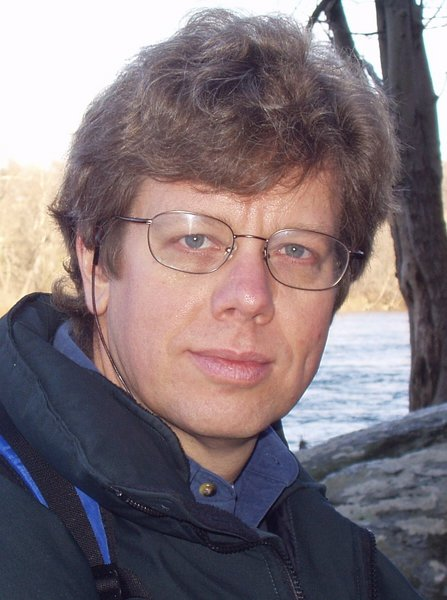
\includegraphics[width=0.5\textwidth]{guido.jpg}
%\end{block}
\end{column}
\begin{column}{.5\textwidth}
%\begin{block}{history}
Concebido en los años 90 por Guido Van Rossum como un sucesor de ABC, un lenguaje de propósito general pensado para la enseñanza y el prototipado.
En el año 2000 aparece Python 2.0
El proyecto sigue siendo orquestado por Guido, lo que le ha hecho merecedor del título de \textit{Benevolent Dictator for Life}.
%\end{block}
\end{column}
\end{columns}
\end{frame}

%------------------------------------------------

\begin{frame}
\frametitle{Conceptos clave}
\begin{itemize}
\item Python es un lenguaje multi-paradigma (oo y programación estructurada)
\item Tipado dinámico y gestión de la memoria automática
\item Es legible
\item Es portable
\item Es integrable
\item Tiene que ser divertido de usar
\end{itemize}
\end{frame}

\begin{frame}
\frametitle{Nobody expects the Python intermission!}
%\begin{block}{Monty Python}
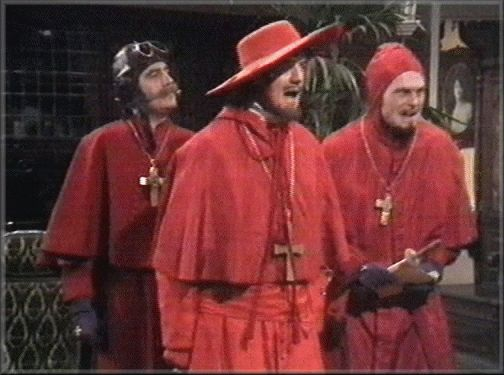
\includegraphics[width=0.9\textwidth]{monty.jpg}
%\end{block}
\end{frame}

%------------------------------------------------
\subsection{Usos}

\begin{frame}
¿Para qué sirve Python?
\end{frame}

\begin{frame}
\frametitle{¿Para qué sirve Python?}
\begin{block}{}
\begin{quote}
Ahá, así que vas a trabajar con algo que nadie sabe muy bien para qué sirve.
\end{quote}
\end{block}
\begin{block}{}
\begin{quote}
Vas a ver que es muy sencillo de utilizar
\end{quote}
\end{block}
\begin{block}{}
\begin{quote}
No conocía ese lenguaje
\end{quote}
\end{block}
\end{frame}

%------------------------------------------------

\begin{frame}
\frametitle{¿Para qué sirve Python?}
\begin{itemize}
	\item Prototipado
	\item Interfaces Gráficas de Usuario
	\item Administración de sistemas
	\item CGI
	\item Scripting
\end{itemize}
\end{frame}

\subsection{Pros y contras}
\begin{frame}
\frametitle{Ventajas de Python}
\begin{itemize}
	\item Es un lenguaje orientado a objetos \textit{opcionalmente}
	\item Es libre
	\item Tiene un gran soporte
	\item Gran espíritu de comunidad
	\item Portabilidad
	\item Potencia
	\item Combinable con otros lenguajes
	\item Fácil de utilizar y de aprender
	\item Sintaxis clara
\end{itemize}
\end{frame}

\begin{frame}
\frametitle{Desventajas de Python}
Rendimiento.
Al ser un lenguaje interpretado, su potencia es menor que la alcanzada con otros como C. Sin embargo, gracias a la traducción del código a un \textit{bytecode} intermedio se ha mejorado notablemente.
\end{frame}

\subsection{¿Quién usa Python?}
\begin{frame}
\begin{block}{}
En adición a los 500,000 usuarios del lenguaje, muchas compañías utilizan el lenguaje en servicios en red y para pruebas de hardware.
\end{block}
\begin{block}{}

\includegraphics[width=0.3\textwidth]{hp.jpg}

\includegraphics[width=0.4\textwidth]{google.png}

\includegraphics[width=0.3\textwidth]{seagate.jpeg}
\end{block}
\end{frame}

\begin{frame}
\frametitle{La Pi de Raspberry Pi}
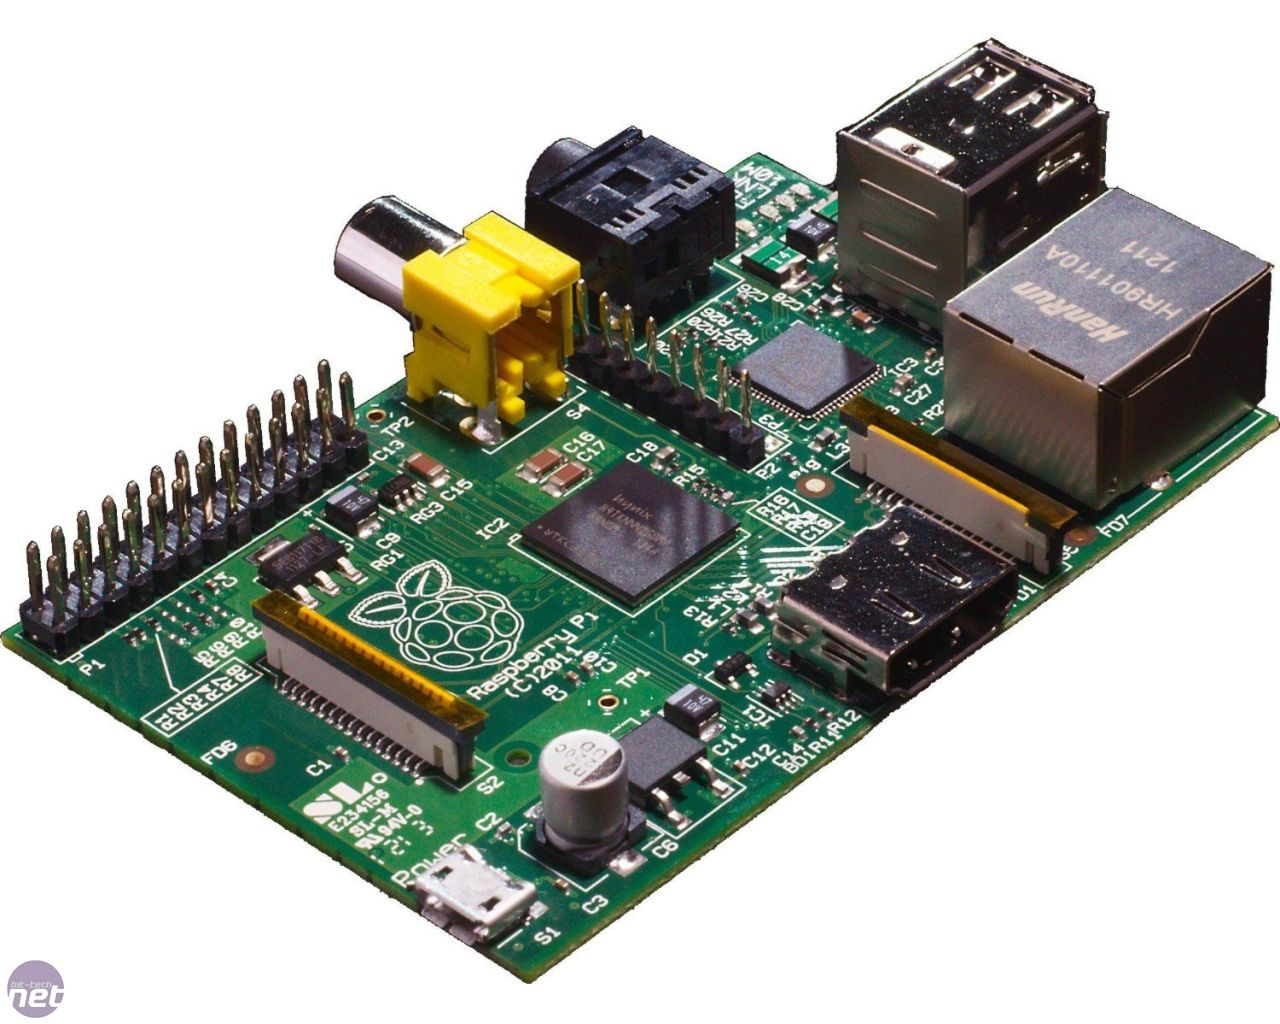
\includegraphics[width=0.9\textwidth]{pi.jpg}
\end{frame}

\section{Tipos de datos}
\subsection{Números}
\begin{frame}
\frametitle{Números}
\begin{columns}[c] % The "c" option specifies centered vertical alignment while the "t" option is used for top vertical alignment

\column{.45\textwidth} % Left column and width
\textbf{Aporta mucha flexibilidad}
\begin{itemize}
\item Enteros
\item Reales
\item ¡Complejos!
\item El límite lo marca la memoria del equipo
\end{itemize}

\column{.5\textwidth} % Right column and width
\textbf{Operaciones con números}
Cualquier operación soportada en C, en adición a nuevas como la suma con truncado (//). Es capaz de trabajar con varias bases de forma natural. La conversión entre números de distinta precisión es `hacia arriba' a menos que se especifique lo contrario.
\end{columns}
\end{frame}

\subsection{Cadenas de texto}
\begin{frame}
\frametitle{Cadenas de texto}
\begin{columns}[c]
\column{.45\textwidth}
En Python son un tipo de secuencia. El lenguaje cuenta con un potente conjunto de utilidades para la manipulación de cadenas. Son elementos inmutables por lo que una vez creados no se pueden modificar. Trabaja con varios tipos de codificación de caracteres.

%\lstset{language=python, showspaces=false}
%\begin{lstlisting}[frame=single, showspaces=false]
%%#!/usr/bin/env python
%print
%\end{lstlisting}
\column{.45\textwidth}
\begin{itemize}
\item Búsqueda por índices: cadena[i]
\item Iteración: for x in cadena
\item Métodos: cadena.capitalize(), cadena.center(), isalnum()\dots
\end{itemize}
%\begin{itemize}
%\item Búsqueda por índices: \verb+cadena[i]+
%\item Iteración: \verb+for x in cadena+
%\item Métodos: \verb+cadena.capitalize()+, \verb+cadena.center()+, \verb+isalnum()+\dots
%\end{itemize}
\end{columns}
\end{frame}

\subsection{¿Cómo funciona la gestión de la memoria?}
\begin{frame}
\frametitle{Gestión de la memoria}
Toda variable en Python almacena una referencia a un dato en la memoria. La gestión de esta se realiza mediante un contador de referencias.\newline
\textbf{Importante}: Si bien las variables no tienen un tipo, los datos almacenados sí, y la conversión no es automática.
\end{frame}

\subsection{Listas y diccionarios}
\begin{frame}
Tercera categoría: mapas..\\
Destacan las listas y los diccionarios.
\end{frame}

\begin{frame}
\frametitle{Listas}
Una lista es una colección de elementos ordenados muy flexible. No importa el tipo de objeto que almacenen (son colecciones de referencias), e implementan muchas de las operaciones que en otros lenguajes son responsabilidad del programador.\\
Son mutables, de longitud variable y orden definido.
Ejemplos de listas:
%\begin{lstlisting}[frame=single, showspaces=false]
%#!/usr/bin/env python
%L1 = [];
%L2 = ['abc', 'is', 'as', 'easy', 'as'];
%L2.append('123');
%\end{lstlisting}
\end{frame}

\begin{frame}
\frametitle{Diccionarios}
Los diccionarios son el tipo más flexible integrado en el lenguaje.\\
Son colecciones de elementos sin orden clasificados por entradas clave-valor. Son mapas mutables.
%%Ejemplos
\end{frame}

\begin{frame}
\frametitle{Trabajo con índices}
Trabajar con índices en Python es mucho más versátil que en otros lenguajes mediante la adición de operadores nuevos:
\begin{itemize}
	\item array[1:]
	\item array[:4]
	\item array[1:3]
	\item array[-1]
	\item array[:]
\end{itemize}
\end{frame}

\subsection{Mutable y no mutable}
\begin{frame}
\frametitle{Para qué sirve tener tipos inmutables y mutables?}
La principal ventaja de contar con ambos tipos de elementos es la flexibilidad de unos y la garantía de \textit{inmovilidad} de los otros.
\begin{center}
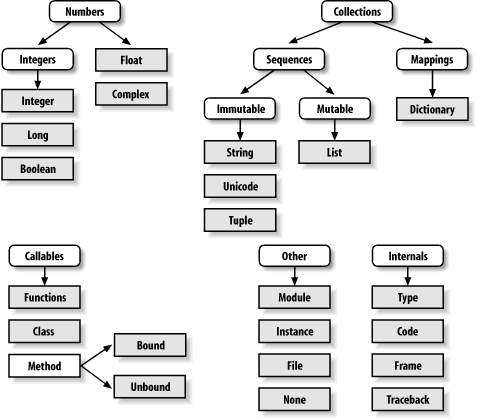
\includegraphics[height=0.7\textheight]{tree.png}
\end{center}
\end{frame}

\section{Control del flujo}
\begin{frame}
\begin{itemize}
\item if, elif, else
\item while
	añade operadores como else
\end{itemize}
\end{frame}

\section{Funciones}
\begin{frame}
Toda función en Python genera una referencia que se almacena en un nombre. Ejemplos:
\end{frame}

\section{Módulos}
\begin{frame}
\frametitle{Módulos}
Un módulo de Python es un paquete de código que permite aumentar la funcionalidad de programas mediante la reutilización de piezas de otros. A grandes rasgos constituyen paquetes de nombres que son cargados (y compilados sin es necesario) en memoria según la funcionalidad que se desee aprovechar de ellos.\\
Fomentan la reusabilidad del código, particionan el espacio de nombres e implementan servicios compartidos o datos.\\
Se utilizan las sentencias \textbf{import} o \textbf{from} para añadir módulos al programa.
\end{frame}

\section{Orientación a objetos}
\begin{frame}
Al ser un lenguaje multiparadigma, la utilización de objetos o no es una decisión delegada al programador. Sin embargo es altamente recomendable utilizar la orientación a objetos debido a los beneficios que supone.
\end{frame}

\begin{frame}
\frametitle{Ejemplo de una clase}
%%Do
\end{frame}

\section{Excepciones}
\begin{frame}
Las excepciones son mecanismos de control de situaciones irregulares dentro del flujo de un programa. Consisten en bloques de código rodeados por las palabras \textbf{try}, \textbf{except} y \textbf{finally}. Se capturan tanto excepciones incluidas en los módulos estándar de Python como aquellas excepciones definidas por el usuario (utilizando \textbf{raise}).
\end{frame}

%------------------------------------------------
\begin{frame}
Demo time!
\end{frame}

\begin{frame}
\frametitle{Impacto en el mundo del desarrollo de software.}
%%XKCD here
\end{frame}

\begin{frame}
\Huge{\centerline{The End}}
\end{frame}

%----------------------------------------------------------------------------------------

\end{document} 